%%This is a very basic article template.
%%There is just one section and two subsections.
\documentclass{article}
\usepackage[utf8x]{inputenc} % работа с utf-8 заработала с такой настройкой
\usepackage[russian]{babel} % Пакет поддержки русского языка
\usepackage[linkcolor=black, colorlinks=true, linktoc=all]{hyperref} % пакет для использования гиперссылок see http://en.wikibooks.org/wiki/LaTeX/Hyperlinks
\setlength{\voffset}{-3cm}
\setlength{\textheight}{24cm}

\usepackage{listings}
\lstset{language=C, basicstyle=\small, keywordstyle=\color{Navy}\bfseries, commentstyle=\color{gray}\slshape}

\usepackage{colortbl}
\definecolor{myyellow}{rgb}{1,1,0.8}
\definecolor{mygreen}{rgb}{0.8,1,0.8}
\definecolor{Navy}{rgb}{0.0,0.0,0.5}
\definecolor{gray}{rgb}{0.05,0.05,0.05}

\ifpdf
% we are running LaTeX, not pdflatex
\usepackage[pdftex]{graphicx}
\usepackage{epstopdf}
\else
% we are running pdflatex, so convert .eps files to .pdf
\usepackage{graphicx}
\fi

\begin{document}
\author{Миннигалиев Т.}
\title{Makefile}


\begin{titlepage}
\begin{center}


\vspace*{7cm} % добавляем пустое место
% Title
\hrulefill \\[1.0cm]

{ \Large \bfseries Описание библиотеки stack\_heap}\\[0.8cm]

\hrulefill \\[1.5cm]

% Author and supervisor
%\begin{minipage}{0.4\textwidth}
%\begin{flushright}
%\large
%Миннигалиев Т.
%\end{flushright}


\vfill

% Bottom of the page
{\large \today}

\end{center}

\end{titlepage}
\newpage
\tableofcontents

\newpage
\section{Назначение библиотеки}
Библиотека stack\_heap предназначена для замены стандартных процедур работы с динамической памятью. Основное отличие этой библиотеки от стандартных средств заключается в том, что библиотека даёт больше возможностей как по контролю за использованием динамической памяти, так и по решению возможных проблем с её утечками.
Библиотека призвана дать примерно те же возможности по отладке, что даёт библиотека dmalloc, но при этом она позволяет решить проблему возврата потерянной памяти не особо разбираясь, где эта память должна быть освобождена.

\section{Основные достоинства библиотеки}
\begin{itemize}
\item Поддержка нескольких куч (это особенно актуально для систем, где есть разные виды памяти).
\item Поддержка вложенных куч - это даёт возможность использовать отдельную кучу для какой-нибудь задачи, а по окончании выполнения задачи уничтожить кучу, не заботясь об утечках памяти.
\item Поддержка возможности сбора статистики по куче (список неосвобождённых указателей, объём общей памяти, объём неосвобождённой памяти).
\item Защита от ошибок программиста. Библиотека постоянно анализирует целостность кучи и в случае обнаружения проблем выдаёт сообщение об ошибке. Также она защищает программиста от повторных освобождений одного и того же указателя.
\item Поддержка произвольного выравнивания. Библиотека позволяет выделять блоки памяти с любым выравниванием (в т.ч. не степенями 2).
\item Портабельность. Библиотека в настоящее время собирается для ОС Linux и для DSP-проектов.
\end{itemize}

\section{Недостатки библиотеки}
\begin{itemize}
\item Библиотека пока что не использует каких-либо специфических структур данных типа binary heap для ускорения поиска подходящего элемента. Т.е. аллокация памяти может занимать время O(n) где n - количество свободных блоков. Таким образом, она плохо подойдёт для применений, где выделяется много маленьких кусочков памяти и где при этом, критично время выделения этой памяти.
\item Одна структура данных (заголовок блока), соответствующая блоку, занимает 24 байта (6 слов) в случае, если отключены отладочные возможности и 36 байт (9 слов) в случае, если отладочные возможности включены. Это также делает применение библиотеки малоцелесообразным, если размеры самих выделяемых кусочков сравнимы с размерами заголовков блоков.
\end{itemize}

\newpage
\section{API библиотеки}
\subsection*{}
\begin{lstlisting}
sth_t * sth_init(
        void * address, 
        unsigned long size, 
        sth_dbg_t *dbg);
\end{lstlisting}
Создаёт новую кучу. Идентификатором кучи будет переменная-указатель на sth\_ctx\_t.
Входные параметры:
\begin{tabbing}
address\quad\= - указатель на начало области памяти, отводимой под кучу\\ 
size \>        - размер области памяти, отводимой под кучу\\
dbg \>         - указатель на отладочную структуру для этой кучи (можно оставлять равным NULL).
\end{tabbing}

\subsection*{}
\begin{lstlisting}
int         sth_set_name(
        sth_t * heap, 
        const char * const name);
\end{lstlisting}
Присваивает куче имя.
Входные параметры:
\begin{tabbing}
heap\quad\=    - указатель на структуру кучи, для которой задаётся имя\\ 
name \>        - указатель на имя кучи
\end{tabbing}
Куче можно присвоить имя. Имеет смысл сделать это, если куч несколько и хочется, чтоб отладочная информация содержала имя кучи. Эта функция будет работать только если куча связана с отладочной структурой.

\subsection*{}
\begin{lstlisting}
sth_dbg_t *sth_dbg_init(
        sth_t * heap, 
        int hash_table_size);
\end{lstlisting}
Инициализирует отладочную структуру.
Входные параметры:
\begin{tabbing}
heap\quad\=    - указатель на структуру кучи, которая будет использоваться для работы отладочной структуры\\ 
hash\_table\_size \>        - размер хэш-таблицы
\end{tabbing}
Отладочная структура при своей работе требует выделения памяти, поэтому ей нужно предоставить указатель на кучу, с которой она будет работать. При этом эта отладочная структура становится отладочной структурой для этой кучи, т.е. допустима такая последовательность создания объектов:
\begin{lstlisting}
sth_t *heap = sth_init(some_address, some_size, NULL);
sth_dbg_t *dbg = sth_dbg_init(heap, 150);
\end{lstlisting}
при этом отладочная функциональность, контекстом которой является структура dbg будет использовать heap в качестве динамической памяти, а сама heap (несмотря на то, что у неё в качестве указателя на отладочную структуру был указан NULL, будет использовать dbg в качестве своей отладочной структуры)

\subsection*{}
\begin{lstlisting}
void sth_pf_init(printf_t pf);
\end{lstlisting}
Входные параметры:
\begin{tabbing}
pf\quad\=    - указатель на функцию, которая имеет прототип в точности соответствующий функции printf\\ 
\end{tabbing}
Такую функцию необходимо предоставить библиотеке, чтоб она могла сообщать об ошибках и выводить другую информацию.

\subsection*{}
\begin{lstlisting}
void    * sth_malloc(
        sth_t * heap, 
        unsigned long size, 
        int align, 
        const char * const file_name, 
        const char * const fn_name, 
        const unsigned line_idx);
\end{lstlisting}
Эквивалент malloc. Не очень удобен, т.к. принимает много параметров, половина из которых не относится к аллокации памяти и служит только для отладки. Поэтому добавлен макрос:
\begin{lstlisting}
#define STH_MALLOC(HEAP, SIZE, ALIGN)     \
        sth_malloc((HEAP),(SIZE),(ALIGN), __FILE__, __FUNCTION__, __LINE__)
\end{lstlisting}

\subsection*{}
\begin{lstlisting}
void      sth_free(
        void * ptr, 
        const char *const file_name, 
        const char *const fn_name, 
        const unsigned line_idx);
\end{lstlisting}
Эквивалент free. Не очень удобен по той же причине, что и sth\_malloc. Поэтому добавлен макрос:
\begin{lstlisting}
#define STH_FREE(PTR) \
        sth_free((PTR), __FILE__, __FUNCTION__, __LINE__)
\end{lstlisting}


\subsection*{}
\begin{lstlisting}
void      sth_print_stat(sth_t * heap);
\end{lstlisting}
Выводит статистику об использовании кучи, о количестве блоков, количестве общей памяти, количестве аллоцированной памяти. Для вывода использует функцию, переданную в библиотеку через sth\_pf\_init.

\subsection*{}
\begin{lstlisting}
sth_stat_t sth_get_stat(sth_t * heap);
\end{lstlisting}
возвращает статистику об использовании кучи в виде структуры.

\subsection*{}
\begin{lstlisting}
void      sth_print_heap_structure(sth_t * heap);
\end{lstlisting}
выводит информацию о структуре кучи (содержимое полей заголовка и блоков памяти кучи).

\newpage
\section{Пример использования}
\subsection{Инициализация, использование, завершение}
\begin{lstlisting}
void init_heaps(gl_dsp_config_t *cfg)
{
    SYS_heap_stat_t hs;
    const int DS_RAM_RESERVED = 100000;
    const int INTERN_RESERVED =   2500;
    const int PM_RESERVED     =   2500;
    const int S_RESERVED      =   2500;

    SYS_HeapStat(&hs, SYS_MemDSRAM);
    int ds_ram_alloc_size = hs.heap_max_cont_free - DS_RAM_RESERVED;
    SYS_HeapStat(&hs, SYS_MemIntern);
    int intern_alloc_size = hs.heap_max_cont_free - INTERN_RESERVED;
    SYS_HeapStat(&hs, SYS_MemPM_RAM);
    int pm_alloc_size = hs.heap_max_cont_free - PM_RESERVED;
    SYS_HeapStat(&hs, SYS_MemSRAM);
    int s_alloc_size = hs.heap_max_cont_free - S_RESERVED;

    void *ptr_dsram  = SYS_malloc(ds_ram_alloc_size, SYS_MemDSRAM);
    void *ptr_intern = SYS_malloc(intern_alloc_size, SYS_MemIntern);
    void *ptr_pm     = SYS_malloc(pm_alloc_size,     SYS_MemPM_RAM);
    void *ptr_s      = SYS_malloc(s_alloc_size,      SYS_MemSRAM);

    sth_pf_init(PrintDbg);

    cfg->heap_ds_ram =
        sth_init(ptr_dsram, ds_ram_alloc_size, NULL);
    cfg->stack_heap_dbg =
        sth_dbg_init(cfg->heap_ds_ram, 129);
    cfg->heap_intern =
        sth_init(ptr_intern, intern_alloc_size, cfg->stack_heap_dbg);
    cfg->heap_pm_ram =
        sth_init(ptr_pm, pm_alloc_size, cfg->stack_heap_dbg);
    cfg->heap_sram =
        sth_init(ptr_s, s_alloc_size, cfg->stack_heap_dbg);
}

void done_heaps(gl_dsp_config_t *cfg)
{
    SYS_free(cfg->heap_sram);
    SYS_free(cfg->heap_pm_ram);
    SYS_free(cfg->heap_intern);
    SYS_free(cfg->heap_ds_ram);
}

void some_function(gl_dsp_config_t *cfg)
{
    const int MEMORY_SIZE = 10000;
    int *memory = STH_MALLOC(cfg->heap_intern, MEMORY_SIZE, 1);
    ..................
    STH_FREE(cfg->heap_intern);
}


\end{lstlisting}
Константы DS\_RAM\_RESERVED и подобные нужны для того, чтоб передать библиотеке не всю память (чтоб GidrOS могла ещё что-то аллоцировать с помощью обычного SYS\_malloc).

\newpage
\subsection{Поиск неосвобождённой памяти}
\begin{lstlisting}
void init_heap(gl_dsp_config_t *cfg)
{
    SYS_heap_stat_t hs;
    const int DS_RAM_RESERVED = 100000;

    SYS_HeapStat(&hs, SYS_MemDSRAM);
    int ds_ram_alloc_size = hs.heap_max_cont_free - DS_RAM_RESERVED;

    void *ptr_dsram  = SYS_malloc(ds_ram_alloc_size, SYS_MemDSRAM);

    sth_pf_init(PrintDbg);

    cfg->heap_ds_ram =
        sth_init(ptr_dsram, ds_ram_alloc_size, NULL);
    cfg->stack_heap_dbg =
        sth_dbg_init(cfg->heap_ds_ram, 129);
}

void done_heap(gl_dsp_config_t *cfg)
{
    SYS_free(cfg->heap_ds_ram);
}

void some_function(gl_dsp_config_t *cfg)
{
    const int MEMORY_SIZE = 10000;
    int *memory = STH_MALLOC(cfg->heap_ds_ram, MEMORY_SIZE, 1);
    ..................
    STH_FREE(cfg->heap_ds_ram);
    sth_print_stat(cfg->heap_ds_ram);
}
\end{lstlisting}
sth\_print\_stat выводит в отладочный поток данных информацию о куче, включая список неосвобожденных блоков с указанием  мест, где они были аллоцированы.

\newpage
\subsection{Создание вложенных куч с использованием stack\_heap }
\begin{lstlisting}
void init_heap(gl_dsp_config_t *cfg)
{
    SYS_heap_stat_t hs;
    const int DS_RAM_RESERVED = 100000;

    SYS_HeapStat(&hs, SYS_MemDSRAM);
    int ds_ram_alloc_size = hs.heap_max_cont_free - DS_RAM_RESERVED;

    void *ptr_dsram  = SYS_malloc(ds_ram_alloc_size, SYS_MemDSRAM);

    sth_pf_init(PrintDbg);

    cfg->heap_ds_ram =
        sth_init(ptr_dsram, ds_ram_alloc_size, NULL);
    cfg->stack_heap_dbg =
        sth_dbg_init(cfg->heap_ds_ram, 129);
}

void done_heap(gl_dsp_config_t *cfg)
{
    SYS_free(cfg->heap_ds_ram);
}

void some_other_function(sth_t * heap)
{
    const int MEMORY_SIZE = 100;
    int *memory = STH_MALLOC(heap, MEMORY_SIZE, 1);
    .........
    int *memory = STH_MALLOC(heap, MEMORY_SIZE, 1);
    .........
    int *memory = STH_MALLOC(heap, MEMORY_SIZE, 1);
}

void some_function(gl_dsp_config_t *cfg)
{
    const int NESTED_HEAP_SIZE = 10000;
    sth_t *nested_heap = STH_MALLOC(cfg->heap_ds_ram, NESTED_HEAP_SIZE, 1);
    
    some_other_function(nested_heap);

    STH_FREE(nested_heap);
}
\end{lstlisting}
В данном примере some\_other\_function намеренно написана некорректно, в ней происходит утечка памяти, но при этом, после возврата в some\_function вся потерянная память возвращается.

В реальности так писать программы нельзя, однако такая функциональность кучи может быть полезна, т.к. иногда (например, при хранении строчек, созданных командой аналогичной strdup) хранить все указатели с целью потом освободить память может быть неоправданно.
\newpage
\section{Описание архитектуры библиотеки}
Библиотека состоит из двух модулей: stack\_heap.c и str\_hash.c
В них размещены следующие классы (см рис.\ref{ris:classes diagram}):
\begin{figure}[h!]
	\center{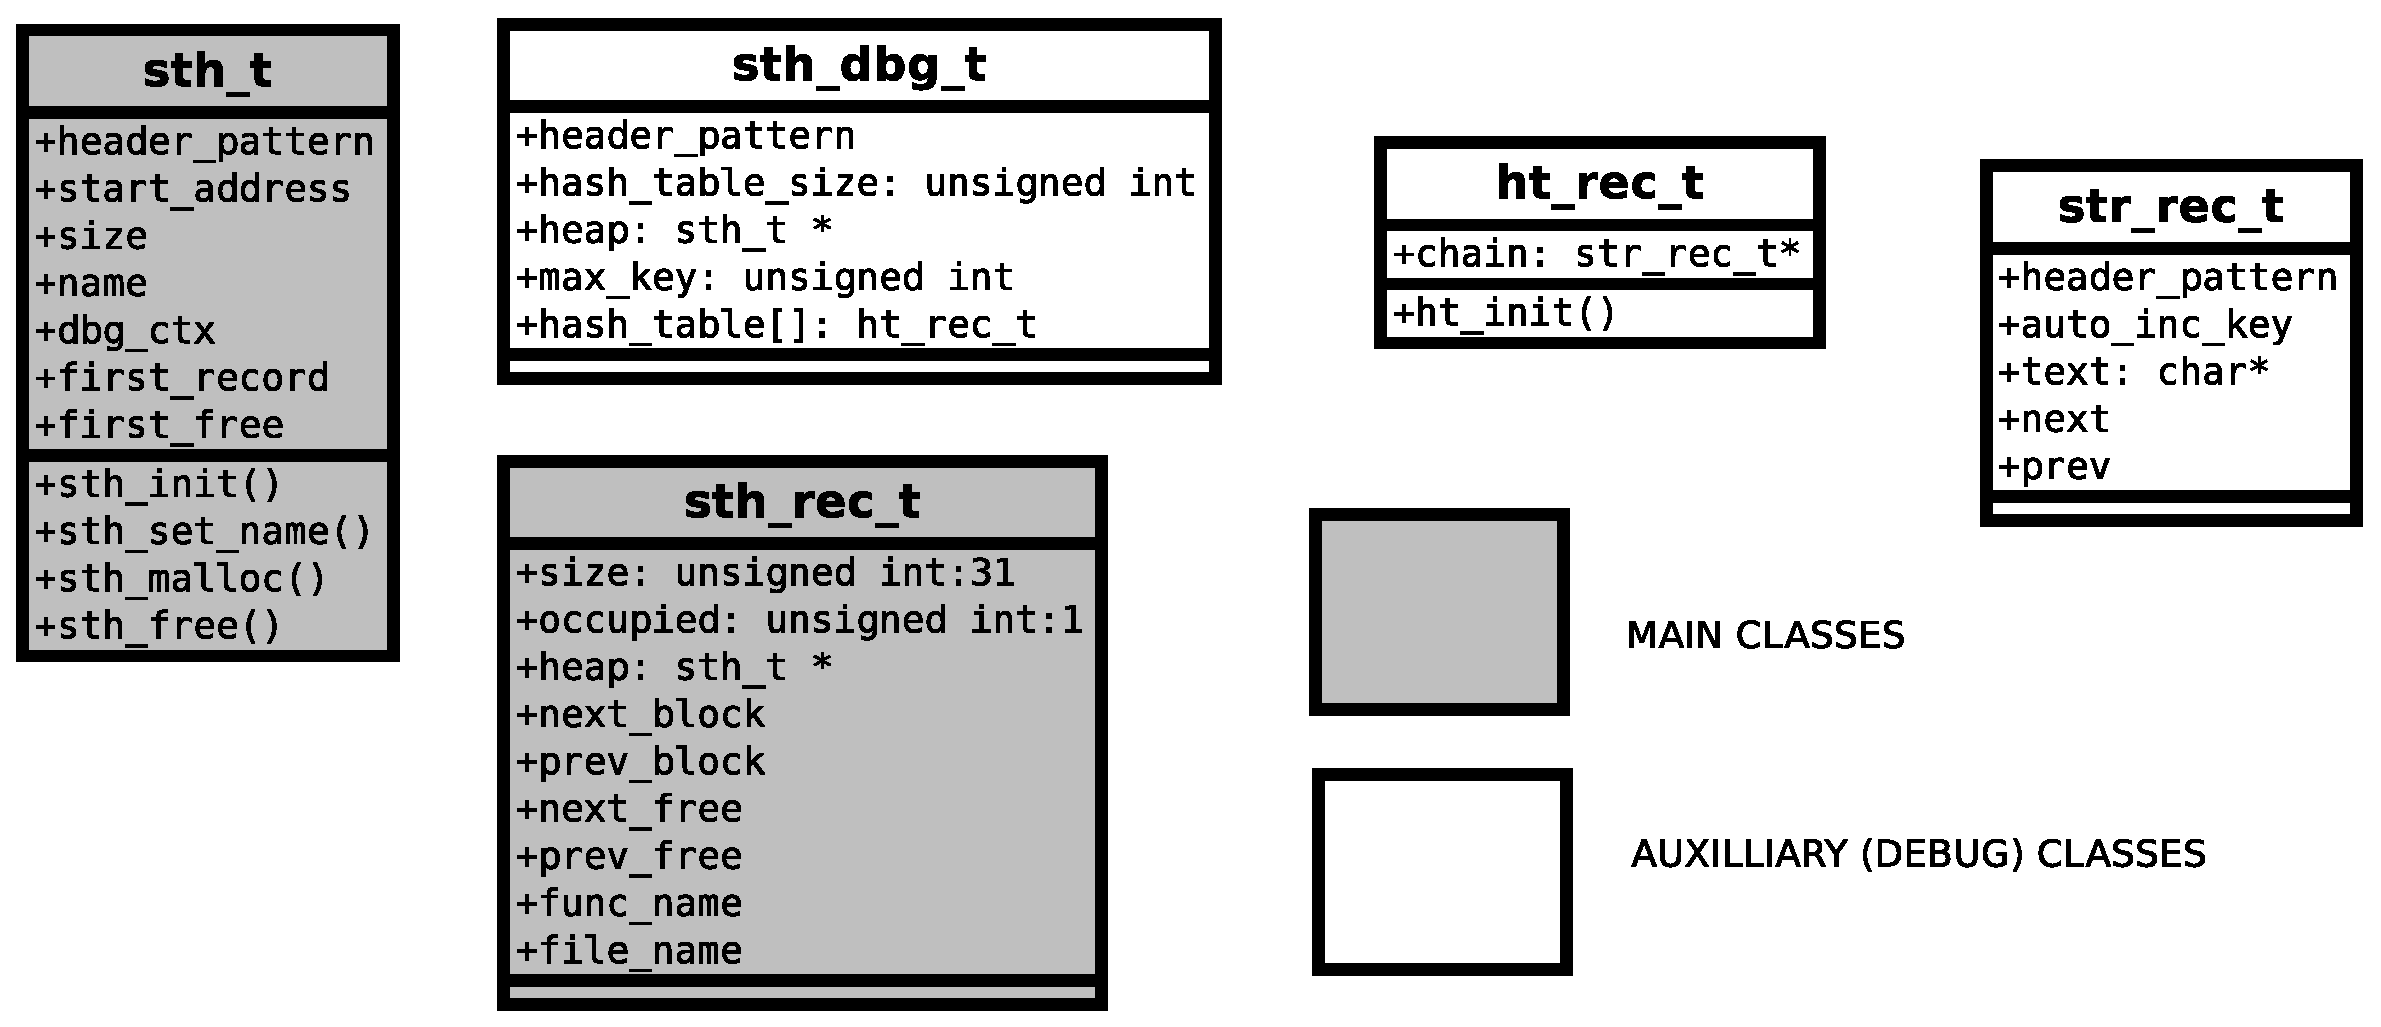
\includegraphics[scale=0.25]{images/classes.eps}}
	\caption{Диаграмма классов}
	\label{ris:classes diagram}
	\end{figure}

После вызова sth\_init, память кучи выглядит как показано на рис.\ref{ris:memory1}
\begin{figure}[h!]
	\center{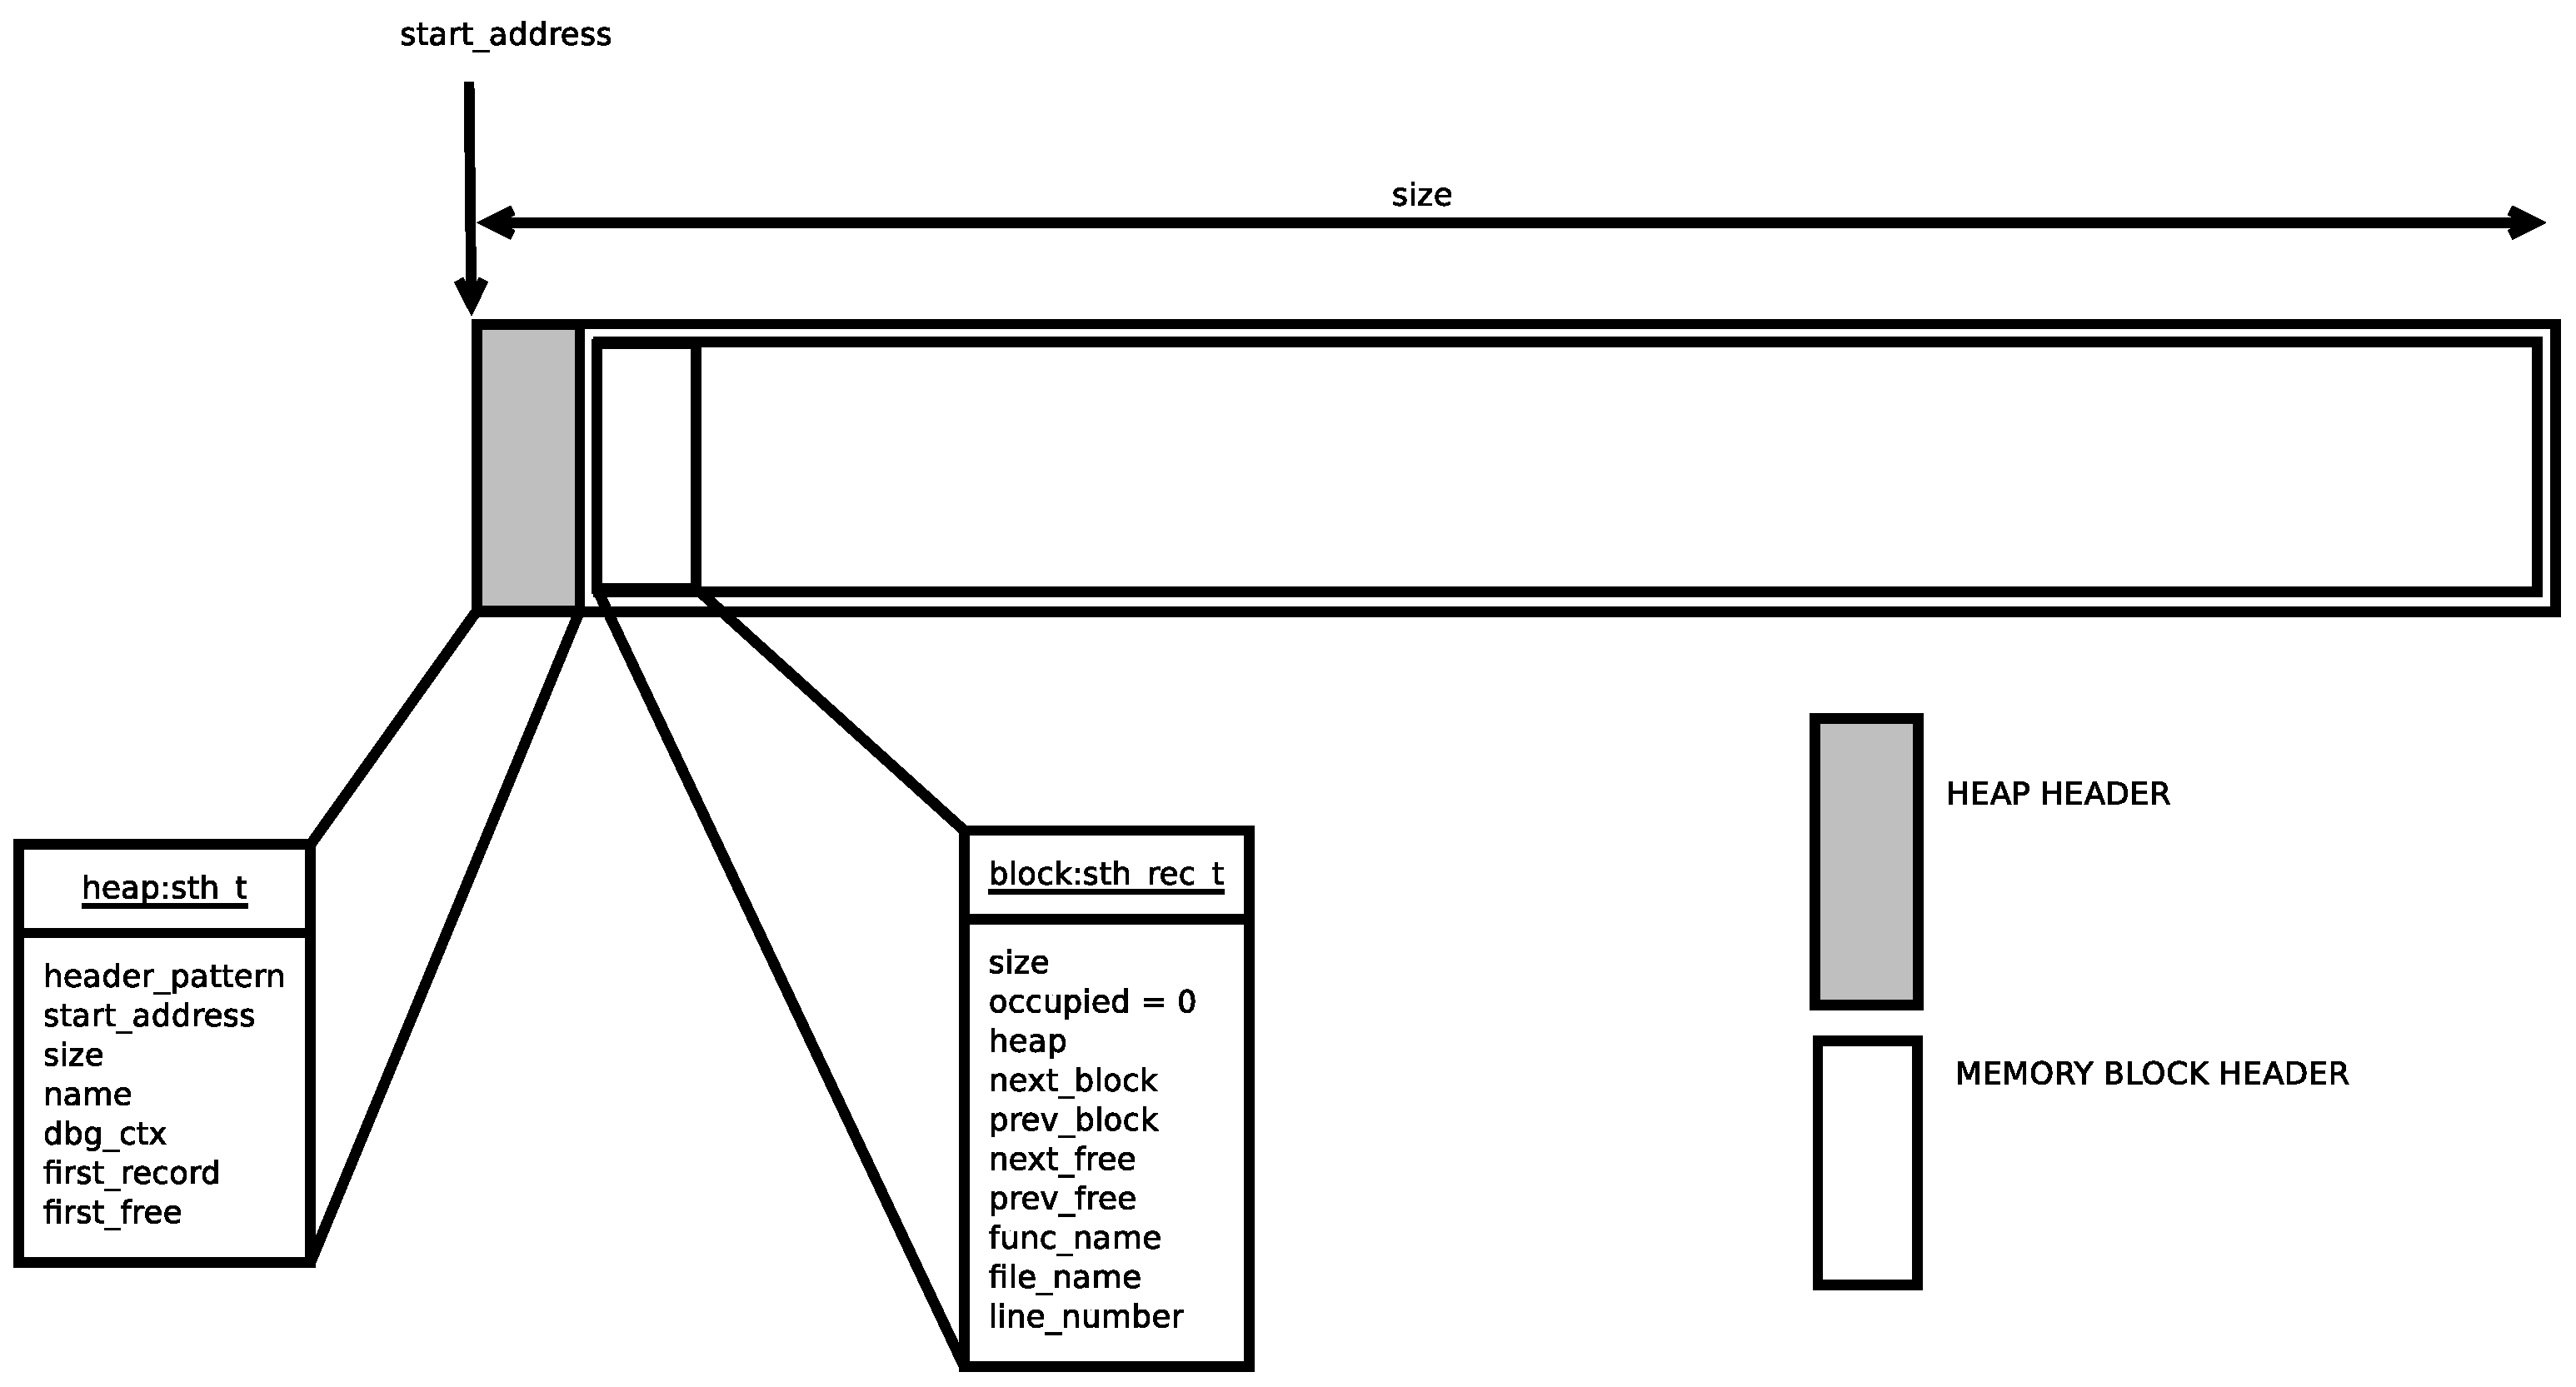
\includegraphics[scale=0.20]{images/memory.eps}}
	\caption{Использование памяти менеджером кучи сразу после инициализации}
	\label{ris:memory1}
	\end{figure}

После выделения первого блока память выглядит как показано на рис.\ref{ris:memory2}
\begin{figure}[h!]
	\center{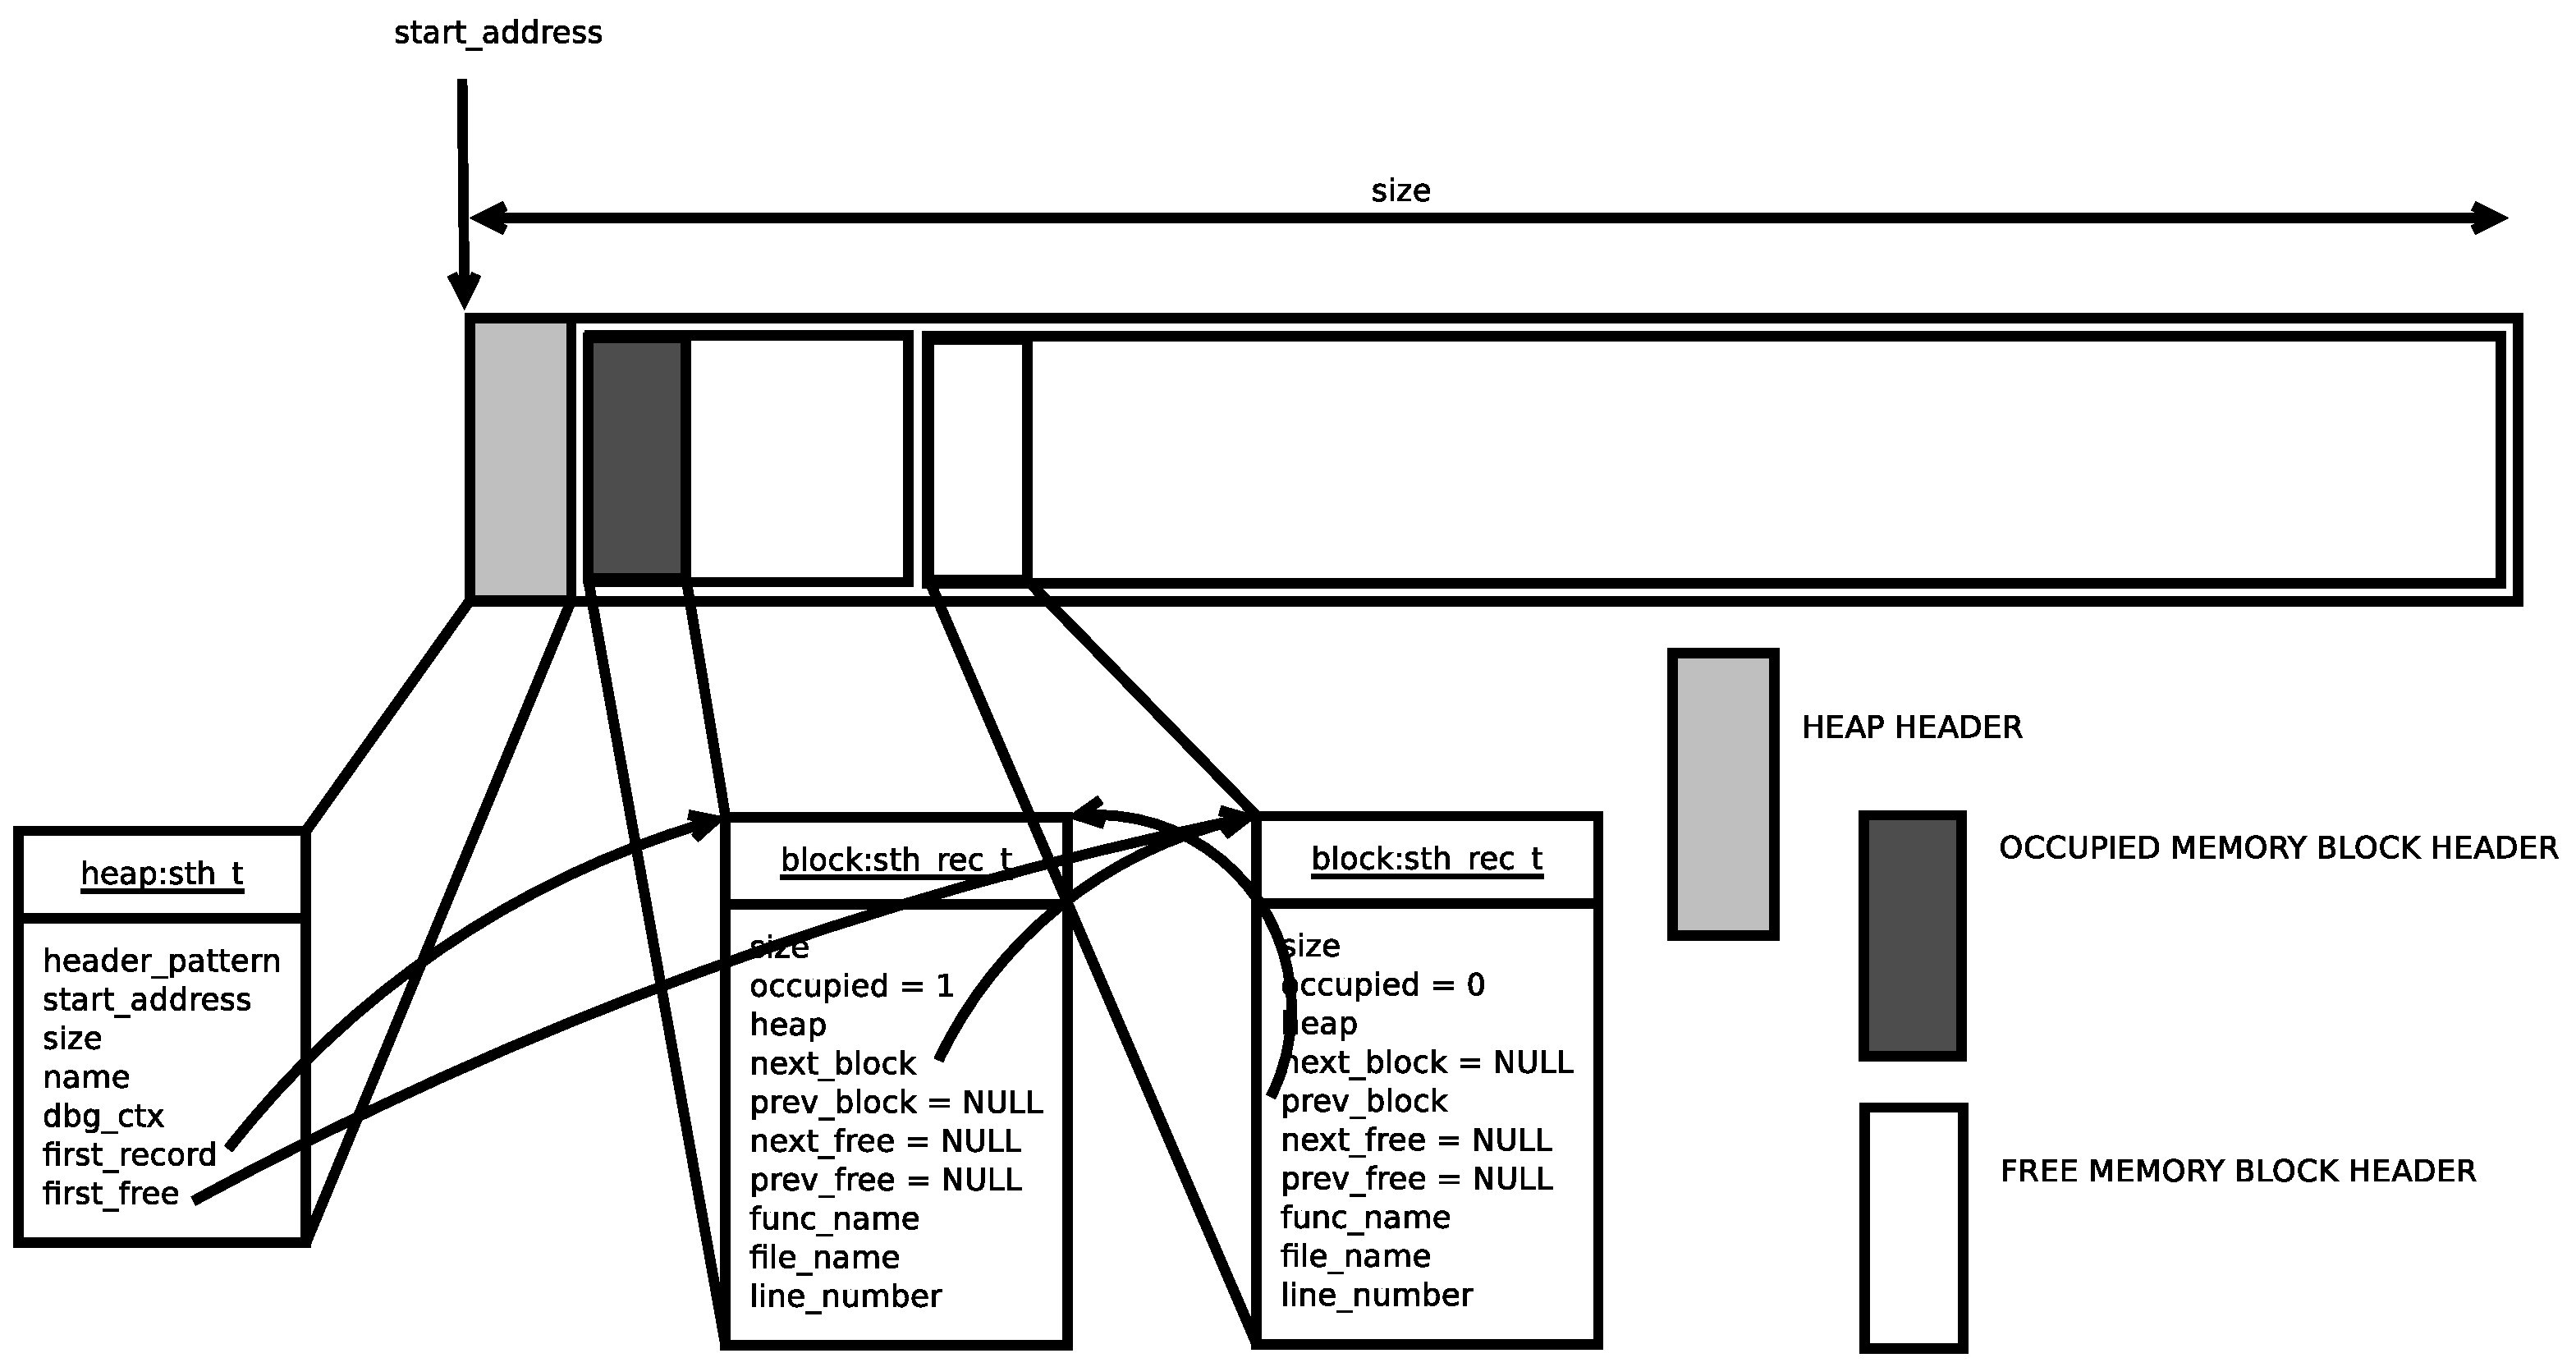
\includegraphics[scale=0.20]{images/memory1.eps}}
	\caption{Использование памяти менеджером кучи после выделения первого блока}
	\label{ris:memory2}
	\end{figure}

\newpage
В случае, если отладочные функции не включены (например, библиотека скомпилирована с опцией  STH\_NO\_DEBUG\_INFORMATION), то будут искользоваться только классы sth\_t и sth\_rec\_t.

В случае, если отладочные функции включены, то для выделения памяти под экземпляры дополнительных классов 
будет использоваться функция sth\_malloc.

Смысл дополнительных классов в том, чтоб организовать такую структуру данных, чтоб каждую строчку хранить только один раз (т.е. например, если будет необходимо 3 раза сохранить в памяти строчку <<complex\_signal.c>> то при первом вызове функции 
\begin{lstlisting}
const char * ht_reg_string(
    const char * const      text,
    struct sth_dbg_tag * dbg);
\end{lstlisting}
под эту строчку действительно будет выделена память и будет возвращён указатель на выделенную строчку, но при последующих вызовах выделяться память не будет, а будет возвращаться указатель на существующую строчку).

Такое поведение достигается за счёт использования хэш-таблицы: для каждой регистрируемой строчки считается значение хэш-функции (для этого перемножаются все символы строчки кроме завершающего нулевого и делятся с остатком на размер хэш-таблицы (задаётся в функции sth\_dbg\_init). Соответствующая строчка хэш-таблицы содержит указатель на список, элементами которого являются строки с одинаковым значением хэша. Т.к. вероятность одинакового значения хэша (при разном содержимом) мала, то поиск внутри списка занимает мало времени (поиск же в хэш-таблице занимает только время, необходимое для расчёта хэш-функции).

\begin{figure}[h!]
	\center{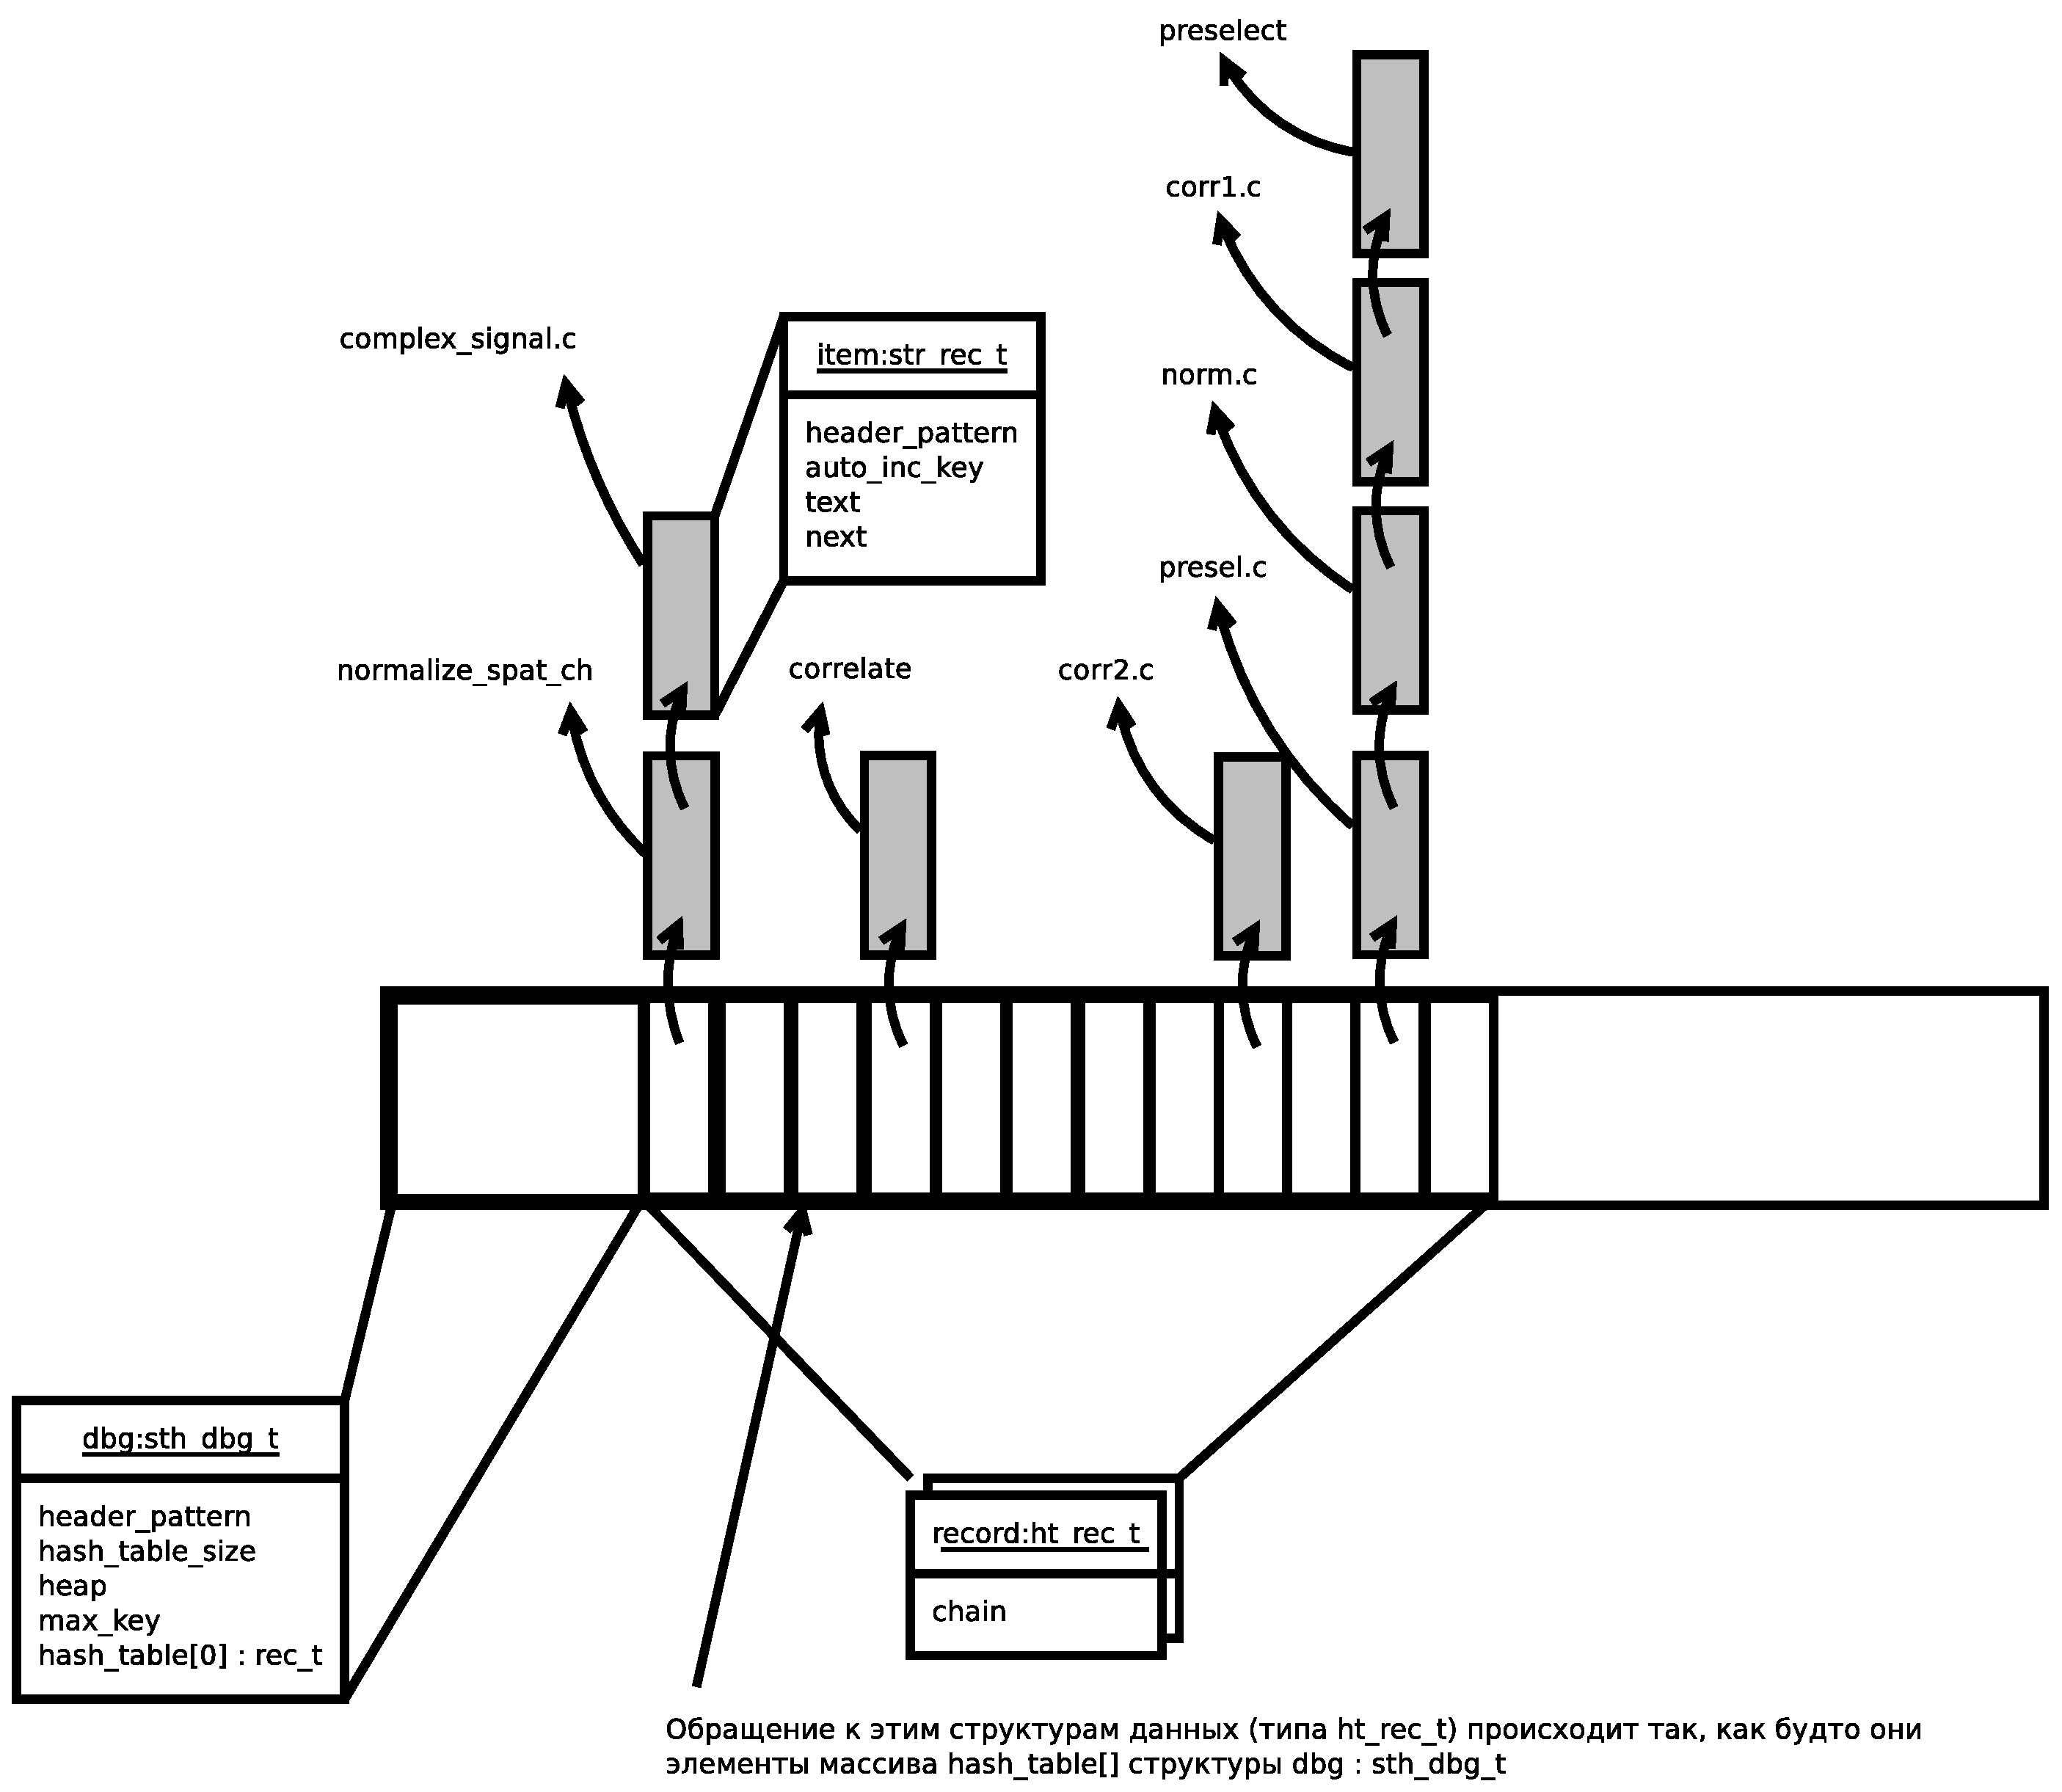
\includegraphics[scale=0.25]{images/hash-table.eps}}
	\caption{Устройство хэш-таблицы}
	\label{ris:hash-table}
	\end{figure}

\newpage
\begin{figure}[h!]
	\center{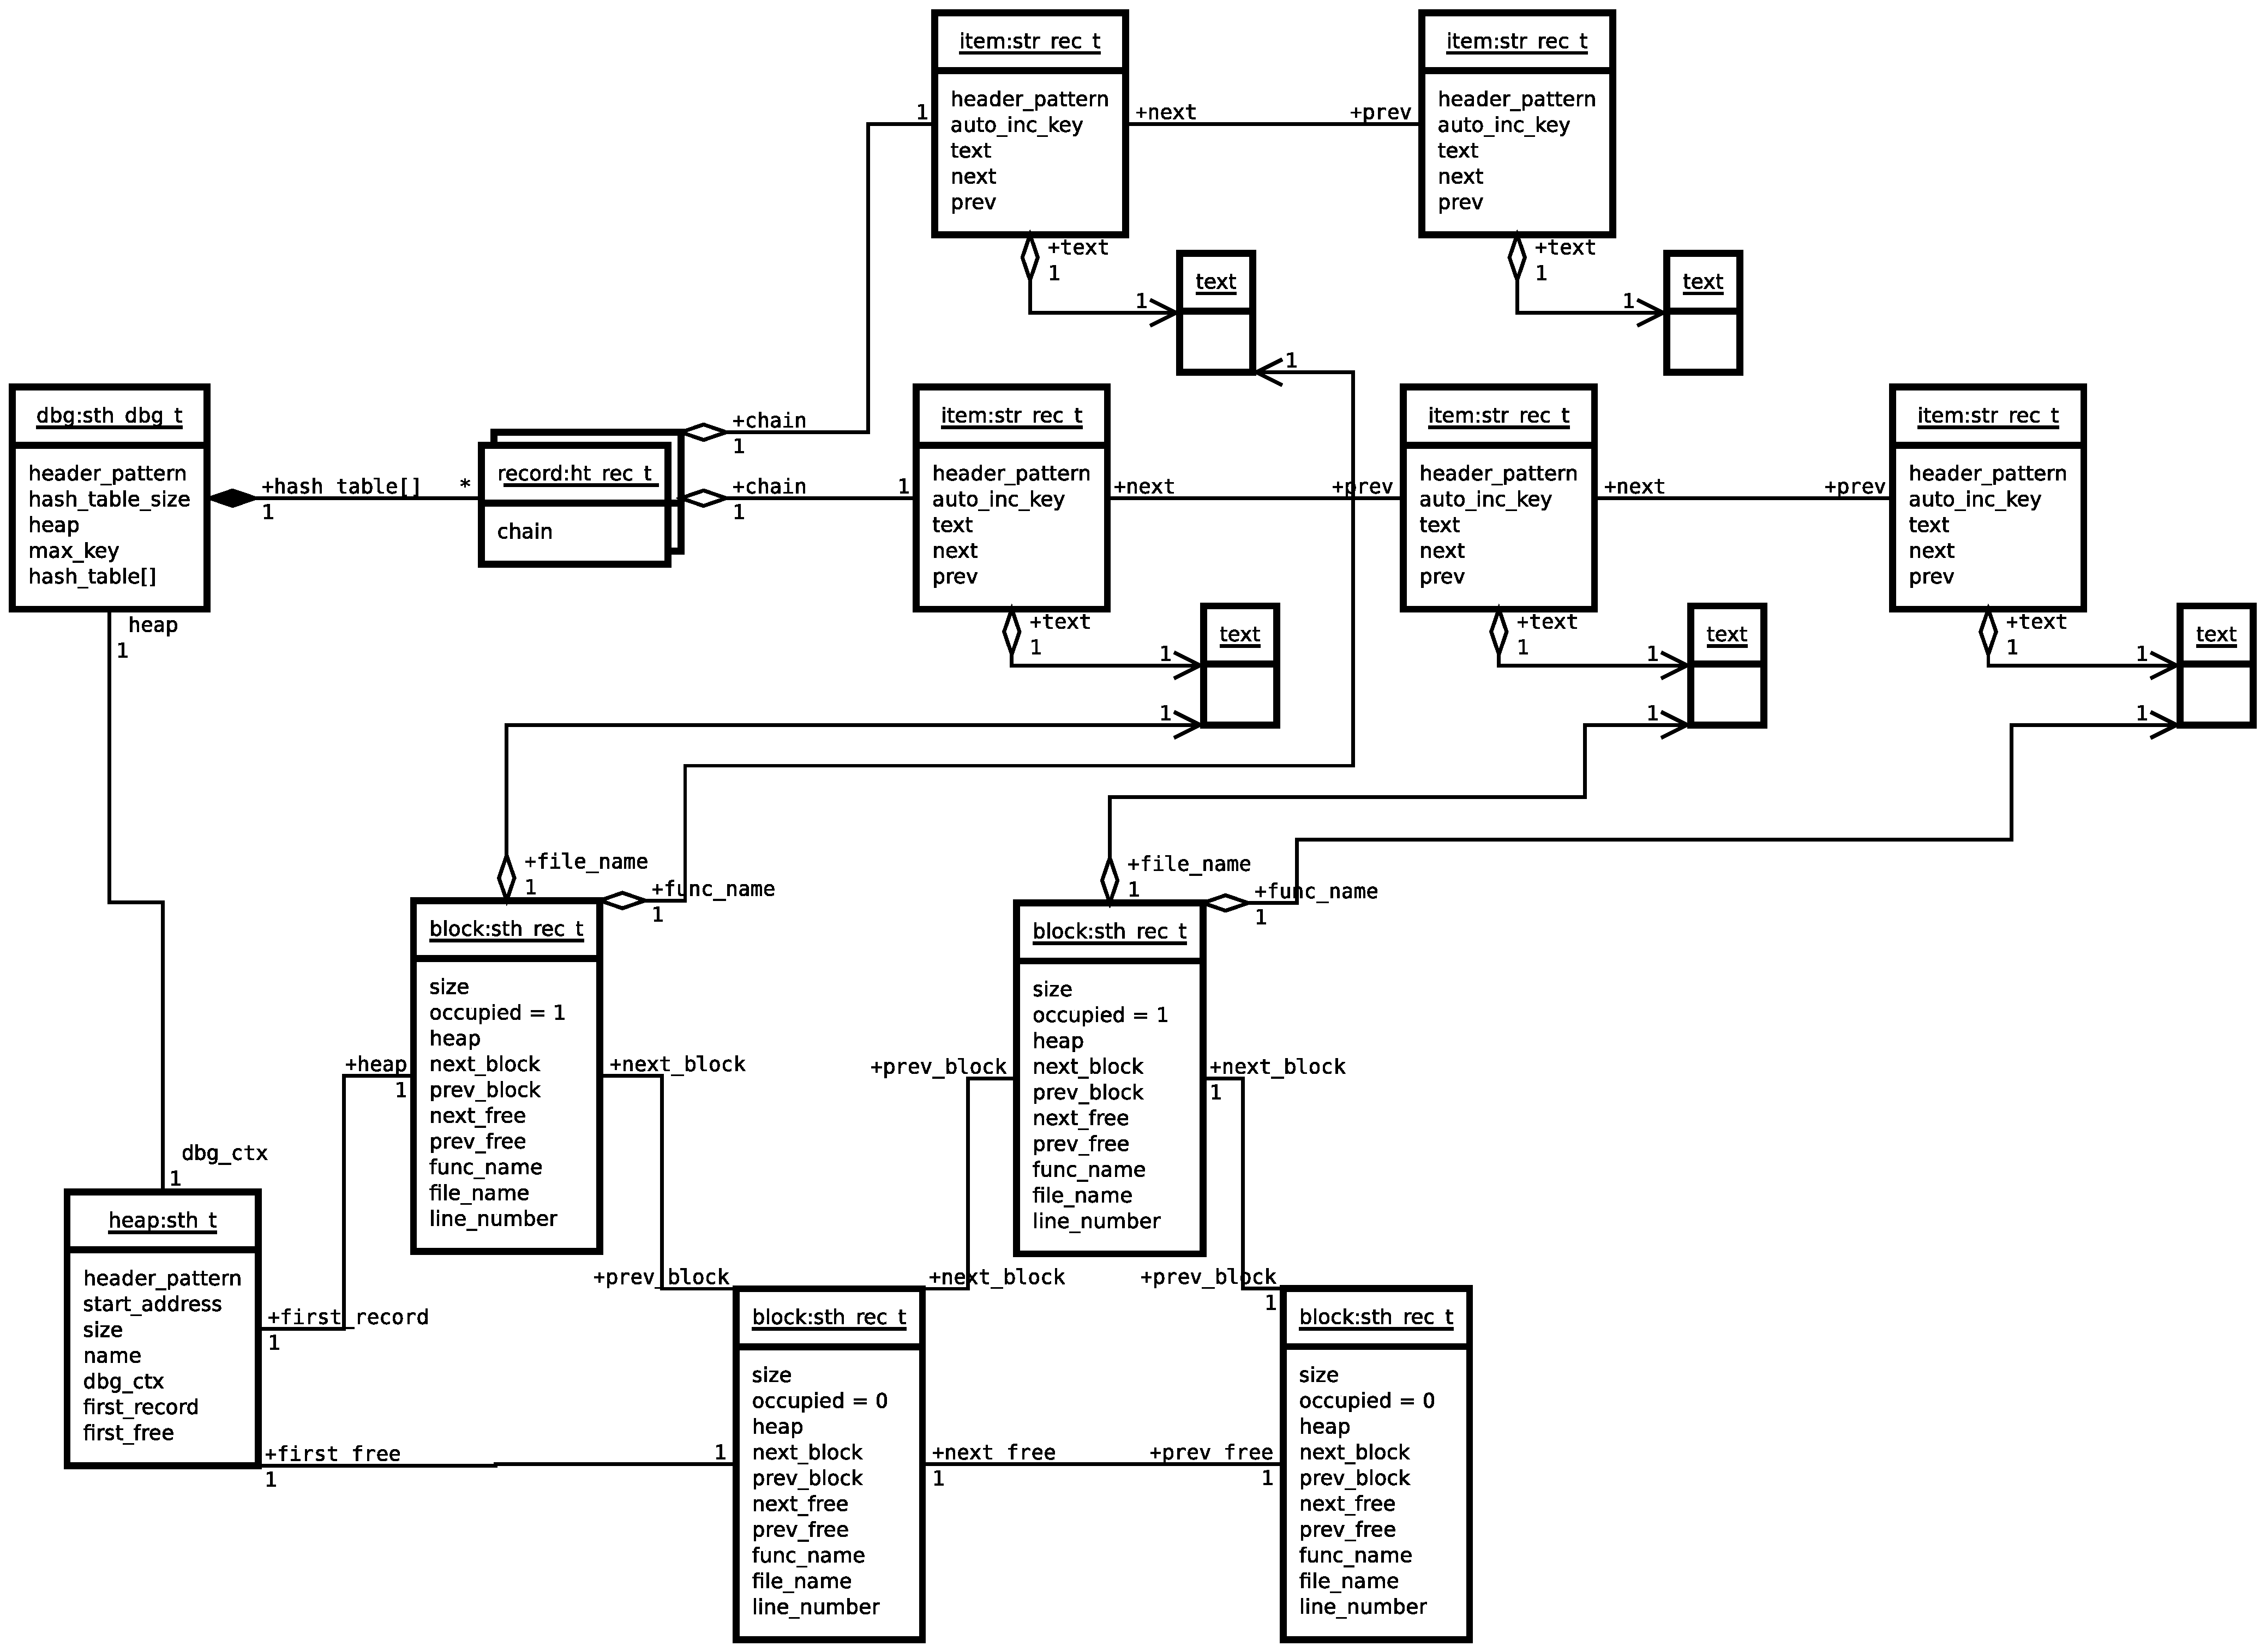
\includegraphics[scale=0.30, angle=90]{images/heap-objects.eps}}
	\caption{Диаграмма объектов}
	\label{ris:object-dia}
	\end{figure}

\newpage
\section{Лист изменений документа}

\begin{tabular}{|l|l|c|} \hline
Дата & Фамилия И.О. & Примечание \\ \hline
17 декабря 2012 & Миннигалиев Т.А. & Начальная ревизия \\ \hline
 &  &  \\ \hline
\end{tabular}
\end{document}
